% MODULO DE DISEÑO =====

\section*{1. Encuesta para Personas Oyentes}
\label{anexo:encuesta_oyentes}

\begin{enumerate}
    \item \textbf{Información Básica}
    \begin{itemize}
        \item Edad
        \begin{itemize}
            \item 18-24
            \item 25-34
            \item 35-44
            \item 45-54
            \item 55+
        \end{itemize}
        \item Género
        \begin{itemize}
            \item Masculino
            \item Femenino
            \item Otro / Prefiero no decir
        \end{itemize}
        \item Lugar de Nacimiento
        \begin{itemize}
            \item Guatemala
            \item Extranjero
        \end{itemize}
        \item Profesión
        \begin{itemize}
            \item (Espacio para respuesta abierta)
        \end{itemize}
    \end{itemize}

    \item \textbf{Conocimiento y Experiencia con la Lengua de Señas}
    \begin{itemize}
        \item ¿Sabes qué es Lensegua?
        \begin{itemize}
            \item Sí
            \item No
        \end{itemize}
        \item ¿Tienes algún conocimiento de la lengua de señas?
        \begin{itemize}
            \item Básico
            \item Medio
            \item Avanzado
            \item Ninguno
        \end{itemize}
        \item ¿Conoces a alguien que sea sordo?
        \begin{itemize}
            \item Sí
            \item No
        \end{itemize}
        \item ¿Cómo te comunicarías con una persona sorda?
        \begin{itemize}
            \item Por mensajes escritos
            \item Señalando lo que quiero decir
            \item Usando Lensegua
            \item No sabría cómo hacerlo
        \end{itemize}
        \item ¿Cuáles consideras que son los principales desafíos que enfrentan las personas con discapacidad auditiva diariamente?
        \begin{itemize}
            \item (Espacio para respuesta abierta)
        \end{itemize}
    \end{itemize}

    \item \textbf{Señas Chapinas}
    Es una aplicación para traducción de LENSEGUA (Lengua de Señas Guatemalteco) a texto o voz.
    \begin{itemize}
        \item ¿Qué tan relevante consideras una aplicación de traducción de lengua de señas para tu vida diaria?
        \begin{itemize}
            \item Muy relevante
            \item Algo relevante
            \item Poco relevante
            \item Nada relevante
        \end{itemize}
        \item ¿Cuáles serían tus principales motivaciones para usar una aplicación de traducción de lengua de señas? (Selecciona todas las que apliquen)
        \begin{itemize}
            \item Comunicación con amigos/familiares sordos
            \item Curiosidad personal
            \item Requerimientos laborales
            \item Actividades voluntarias
            \item Otras: \underline{\hspace{5cm}}
        \end{itemize}
        \item ¿En qué situaciones te gustaría usar la aplicación? (Selecciona todas las que apliquen)
        \begin{itemize}
            \item Trabajo
            \item Educación
            \item Actividades sociales
            \item Voluntariado
            \item Otras: \underline{\hspace{5cm}}
        \end{itemize}
    \end{itemize}

    \item \textbf{Aplicaciones Móviles}
    \begin{itemize}
        \item ¿Qué características consideras más importantes en una aplicación móvil? (Selecciona todas las que apliquen)
        \begin{itemize}
            \item Facilidad de uso
            \item Velocidad y rendimiento
            \item Diseño atractivo
            \item Funciones de accesibilidad
            \item Otras: \underline{\hspace{5cm}}
        \end{itemize}
    \end{itemize}

    \item \textbf{Comentarios Adicionales}
    \begin{itemize}
        \item ¿Cuáles características consideras esenciales para una aplicación de traducción de lengua de señas y por qué?
        \begin{itemize}
            \item (Espacio para respuesta abierta)
        \end{itemize}
    \end{itemize}
\end{enumerate}

\section*{2. Preguntas para Entrevistas a Personas Sordas}

\begin{enumerate}
    \item \textbf{Información Básica}
    \begin{itemize}
        \item Edad
        \item Lugar de nacimiento
        \item Profesión
    \end{itemize}

    \item \textbf{Comunicación}
    \begin{itemize}
        \item ¿Qué tipo de sordera tienes?
        \item ¿Cómo hablas con una persona oyente que no sabe LENSEGUA?
        \item ¿Utilizas tu teléfono para comunicarte con personas oyentes? ¿Cómo?
    \end{itemize}

    \item \textbf{Señas Chapinas}
    Es una aplicación para traducción de LENSEGUA a texto o voz.
    \begin{itemize}
        \item ¿Cuándo usarías la aplicación?
    \end{itemize}

    \item \textbf{Aplicaciones Móviles}
    \begin{itemize}
        \item ¿Usas mucho las aplicaciones en tu teléfono?
        \item ¿Cuáles son tus aplicaciones más utilizadas? ¿Por qué?
        \item ¿Qué hace que una aplicación sea fácil de usar para ti?
        \item ¿Hay algo que no te guste o te sea difícil en las aplicaciones?
    \end{itemize}

    \item \textbf{Comentarios Adicionales}
    \begin{itemize}
        \item ¿Qué es lo más importante que esperarías de la aplicación Señas Chapinas?
    \end{itemize}
\end{enumerate}






% MODULO DE ARQUITECTURA =====
\section*{3. Carta de Solicitud de Acceso a la VPN}
\addcontentsline{toc}{section}{Carta de Solicitud de Acceso a la VPN}
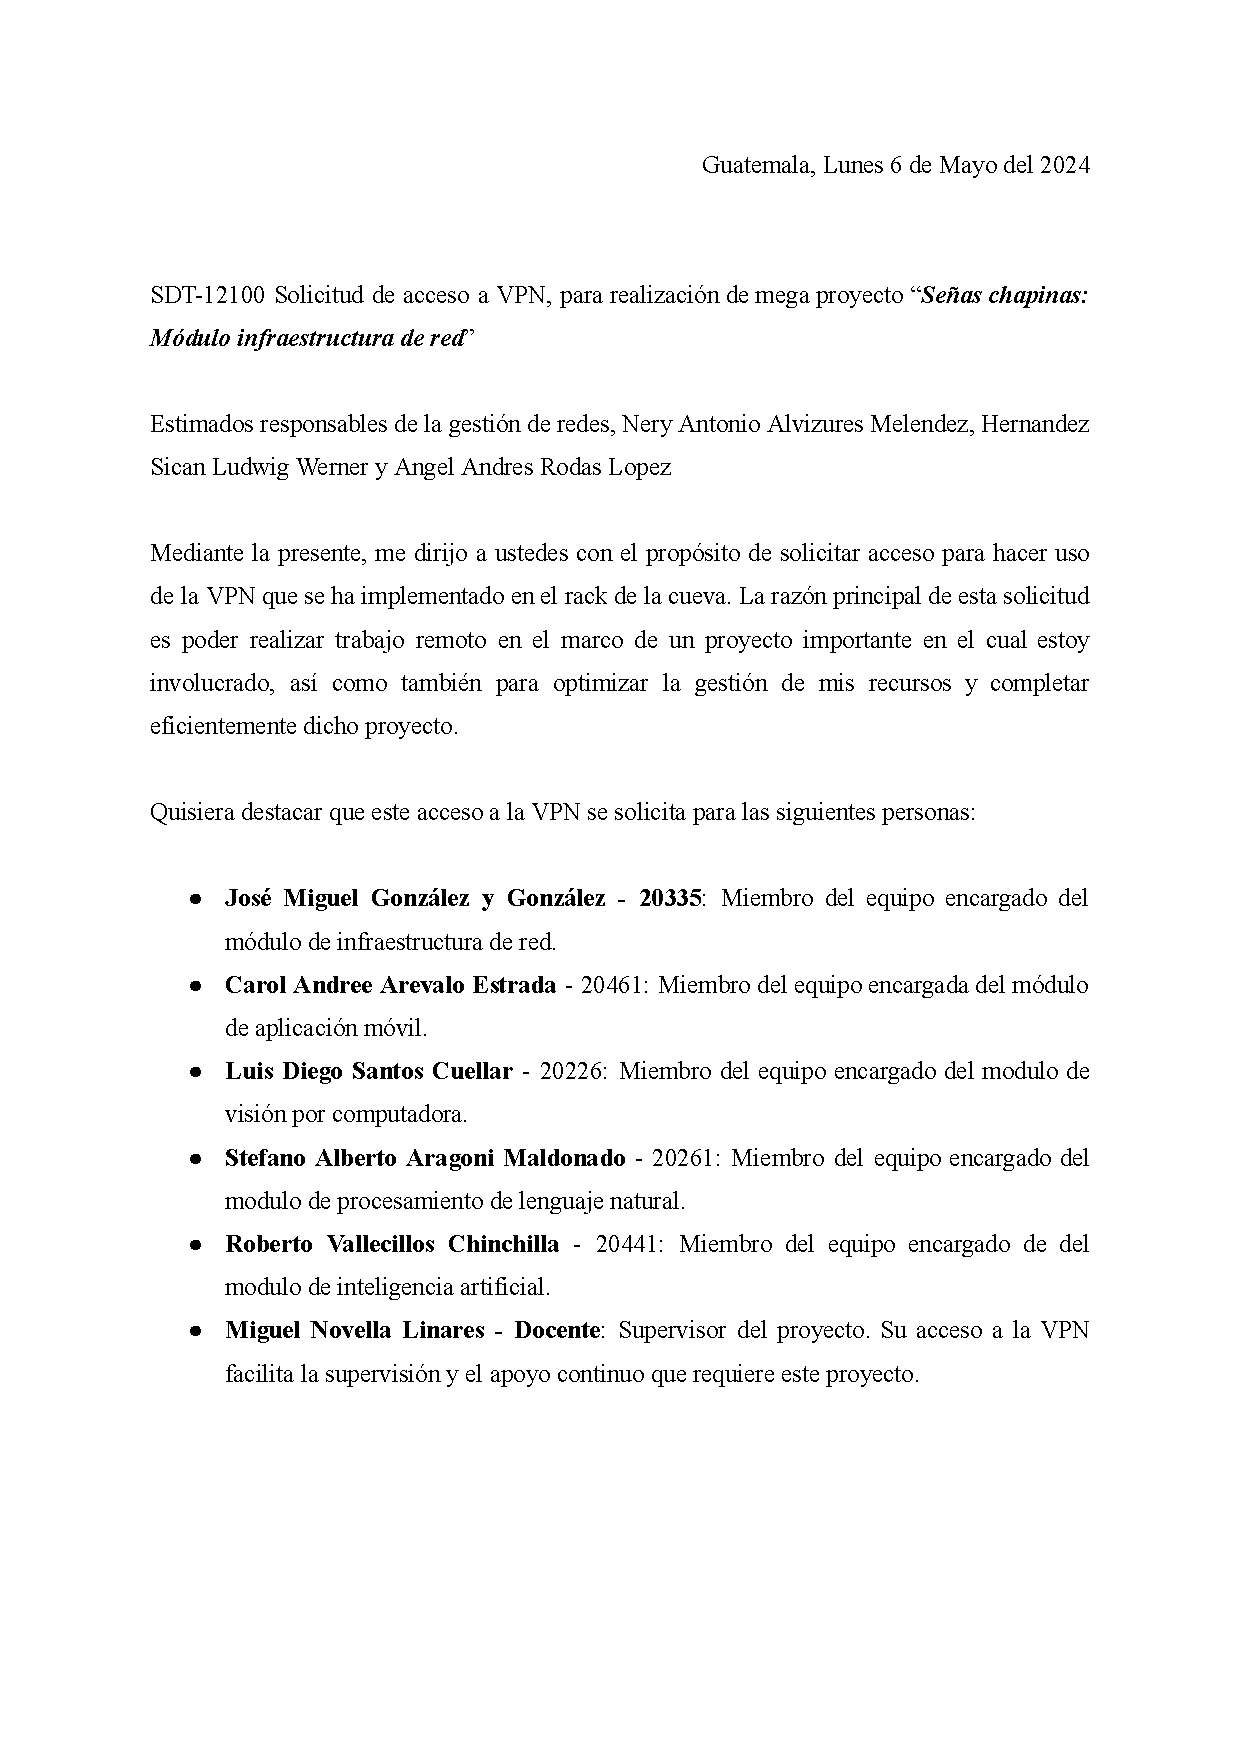
\includepdf[pages=-]{figuras/solicitud_acceso_VPN.pdf}



